\chapter{\texorpdfstring{METHODOLOGY}{}} %upper case only

This chapter outlines the methodology that guided this project exploring identity negotiations, the relationship between immigrant parents and their children (and vice versa), as well as the influence of retrospective storytelling on the process of identity negotiation. Rooted in a constructivist interpretive paradigm, I recognize that reality is co-constructed through individuals’ lived experiences. The stories participants shared, both about themselves and about others, are shaped by their personal experiences, perceptions, and sense-making processes. These narratives are further interpreted through my own positionality as a researcher, particularly as I situate individual stories within broader family relationships and intergenerational contexts. 

As I provide an insider's perspective, I bring a situated perspective to examine the identity development and negotiation within Pakistani immigrant families who navigate life between two cultural contexts and often feel partial belonging in both cultures. I focused on the content and process of retrospective storytelling through which individuals and families articulated identity gaps, negotiated cultural expectations, and made sense of challenges over time. 

I adopted an arts-based (ABR qualitative) research approach through poetic inquiry and used Episodic Narrative In-Depth Interviews (ENI) for data collection. ENI draws on the triangulation of narrative inquiry, in-depth interviews, and episodic interviews, enabling participants to move fluidly between storytelling and reflection while expanding both the width and depth of the data collected. This method was particularly suited to capturing layered experiences of identity negotiation across time.

Consistent with the ABR qualitative approach, poetic inquiry was used to analyze the in-depth episodic narrative interviews of Pakistani American families. Poetic transcripts were developed from the original interview texts, allowing participants’ language, emotional rhythms, and narrative structures to remain central to the analytic process (Faulkner 2025, 2019). As a social justice-oriented method, poetic inquiry provided a participatory and ethical means of amplifying marginalized voices while honoring the complexity of lived experiences \citep{gioiachiltonArtsBasedResearchPractice2014}.  Through storytelling and narrative inquiry, the study provides a unique lens to investigate the lived experiences of these families in times of stress, change, and uncertainty. The study also explores the challenges inside and outside the home based on disproportionate exposure between the first two generations of immigrants to the US culture and Pakistani cultural values.

Poetic transcription is the practice of crafting interview transcripts in a careful, relational, and ethically attentive manner that foregrounds participants’ lived experiences while preserving the affective and relational dimensions of meaning through an evocative, coherent storyline \citep{faulknerPoeticPortraitsOlder2026, faulknerComposingPoemsUsing2024, faulknerPoeticInquiryCraft2019}. This approach allowed me to capture the ways Pakistani American parents and children co-constructed meaning, navigated identity, and reinterpreted family narratives across various life stages, highlighting themes of resilience, cultural preservation, and intergenerational trauma and negotiation.

\section{Method}

\subsection{In-Depth Episodic Narrative Interviewing (ENI)}

The Episodic narrative interview (ENI) method combines the elements of three qualitative research methods: semi-structured interviews, narrative inquiry, and episodic interviews. Introduced by Mueller in 2019, ENI is tightly focused on specific phenomena, which in this study is identity negotiation among immigrant families. This approach offered participants a choice in sharing the content and details of their stories and served as an entry point into narrative focused research. An episodic narrative interview approach honors individual stories of experience and constitutes a manageable yet rigorous way of collecting and analyzing narrative accounts \citep{muellerEpisodicNarrativeInterview2019}.

Using ENI allowed me to capture the voices of participants who are marginalized both broadly and within minority populations as a distinct subgroup, enabling them to share their experiences in detail. As Mueller explains, drawing on the work of \citet{flickEpisodicInterviewSmall1997}, “the episodic interview method is developed in alignment with the psychological claim that memories about experiences are tied to concrete circumstances, which include a combination of time, space, situation, and events that form episodes within an individual’s life” \citep[p.~3-4]{muellerEpisodicNarrativeInterview2019}. Guided by this approach, I examined participants’ identity narratives through the material frame of CTI, the fifth identity layer introduced by \citep{kuiperCommunicationTheoryIdentity2021}.

The material frame foregrounds how identity is shaped through embodied and environmental conditions, emphasizing that identity is not only discursively constructed but also materially lived. Specifically, this frame attends to:
\begin{enumerate}[label=(\arabic*)]
\item how physical attributes shape and influence identity;
\item how health conditions and bodily experiences inform identity negotiations; and
\item how territory, space, and environmental contexts shape individuals’ sense of self and belonging
\end{enumerate}


ENI was particularly well-suited to examining the material frame, as participants’ memories were anchored in concrete moments situated in specific places, bodies, and institutional environments. This alignment allowed for an analysis of how material conditions such as migration status, racialized bodies, educational spaces, homes, and neighborhoods; intersect with personal, relational, and communal identity layers across participants’ life narratives.

\section{Data Collection}

To examine identity negotiation across generations, participants were purposefully selected from three generations within Pakistani American families: parents (first-generation) and children (one-and-a-half and second-generation). Multi-generational perspectives enabled me to capture intergenerational sense-making processes and provided a more comprehensive understanding of how identities are negotiated within family contexts. Participants represented three primary generational groups; first-generation immigrant parents, one-and-a-half (1.5) generation, and second-generation adult children (18 years and over).

\subsection{Sampling}

I used the non-random sampling techniques of purposive sampling and snowball sampling to recruit individuals from the families of first-generation Pakistani immigrants in the US.

\subsection{Recruitment}

All study procedures were reviewed and approved by the Institutional Review Board (IRB) of Bowling Green State University, and the study was conducted in accordance with ethical standards for research involving human participants (IRBNet ID \#2234570). 

All the participants were recruited using purposive sampling and snowball sampling, a strategy particularly appropriate for accessing immigrant and marginalized populations \citep{suriPurposefulSamplingQualitative2011}. Initial contacts were made through Pakistani American communities on Facebook, local mosques, professional networks, and informal family and social connections. Participants were invited to share the study information with eligible family members or acquaintances who met the inclusion criteria. 

Eligibility criteria included:
\begin{enumerate}[label=(\Alph*)]
\item identifying as Pakistani or Pakistani American,
\item residing in the US, and
\item being either a first-generation Pakistani immigrant parent or an adult child born to at least one immigrant parent.
\end{enumerate}

All participants provided informed consent prior to participation either by filling out the demographics form online or a giving verbal consent. In total, I interviewed 24 Pakistani Americans who were either naturalized or citizens by birth, across the three generations of Pakistani American immigrants. 

\subsection{Procedure}

The study was conducted primarily in the Midwest region of the US, including Ohio and Illinois, but some interviews were also conducted in New Jersey, Texas, and Washington, D.C.

Snowball sampling was also employed, as participants referred me to others within their networks who met the study criteria. This approach proved useful in reaching families and individuals who might otherwise be difficult to access, particularly given the private and often sensitive nature of topics related to migration, parenting, and identity negotiation.

When an individual expressed interest in participating, meeting times were arranged through phone calls, text messages, and email exchanges. Interviews took place in participants’ homes, online, and in other mutually agreed upon settings of comfort and convenience. Most of the interviews were recorded and transcribed via Zoom with interviewees’ consent; one person responded in writing. However, two participants did not wish to be recorded; in those cases, I took detailed handwritten notes. Informed consent was obtained prior to each interview, and confidentiality was assured through anonymization of all identifying details.

Interviews were semi-structured and conversational in nature, lasting on average 90 minutes (ranging from 60 to 120 minutes). Additionally, many participants (particularly first-generation immigrants) shifted between English and Urdu during their interviews. These bilingual conversations were automatically transcribed through Zoom’s auto-transcript feature. Additional cleaning and formatting of the specific passages was done using ChatGPT as a first pass to remove superfluous sounds and breaks in speech. I familiarized myself with the research guiding the effective use of Al ChatGPT in the process of systematic thematic analysis \citep{naeemThematicAnalysisArtificial2025}. In the second round of cleaning, I listened to the interview and made further edits to preserve meaning and nuance.

\subsection{Demographic of Participants}

The final sample consisted of 24 Pakistani American participants representing first generation,1.5 generation, and second-generation immigrant identities, ranging in age from 19 to 78 years old. Participants reflected diverse educational backgrounds, professional roles, family structures, and migration trajectories. Despite intentional recruitment efforts, it was notably difficult to access and retain male participants across generations. Several men expressed reluctance to participate or to engage deeply in interviews that required emotional reflection and personal disclosure, a challenge consistent with the gendered norms surrounding emotional expression within many South Asian and immigrant cultural contexts. As a result, the sample includes fewer male than female participants.

Interviews were conducted until theoretical saturation was achieved; that is, when additional interviews no longer contributed new conceptual insights relevant to the study’s theoretical framework and research questions \citep{faulknerQualitativeMethodsCommunication2024}. Data saturation in the traditional sense was neither sought nor deemed feasible, given the heterogeneity of the Pakistani American population across regions, migration histories, sectarian, linguistic, ethnic, and socioeconomic differences. Instead, saturation was assessed in relation to recurring patterns of meaning-making, identity negotiation, and narrative sense-making across generations, consistent with qualitative and arts-based research practices. Researchers argue that it is difficult to determine the exact number of interviews needed to reach data saturation in a qualitative study. They suggest that researchers should conduct as many interviews as possible. Additionally, interview questions should be designed in a way that allows multiple participants to answer the same questions. Otherwise, achieving data saturation would be challenging \citep{saundersSaturationQualitativeResearch2018, fuschAreWeThere2015}. 

The sample also includes participants whose migration histories complicate conventional generational classifications. One first-generation participant, Muhammad, was born in the US while his father was pursuing doctoral studies; however, the family returned to Pakistan during his infancy. Muhammad completed his education in Pakistan and later migrated back to the US as an adult following family encouragement, leaving a government position in Pakistan’s provincial agriculture department. Although he holds US citizenship by birth, his lived experiences align closely with first-generation identity negotiations. 	

Additionally, the sample includes intercultural and mixed-race family perspectives. Khan, a first-generation Pakistani participant, is married to an American woman, offering insight into identity negotiation within a Pakistani American interracial marriage. Similarly, one second-generation male participant comes from a mixed-race family in which his parents were international students in the US from India and Pakistan; a Hindu mother and a Muslim father, who met in college, fell in love, and got married against the wishes of their families here in the US.

To protect confidentiality, all participant names used in this study are pseudonyms, and identifying details were modified where necessary. The demographics of the participants mirror the broader demographic makeup of 1st generation Pakistani Americans in table \ref{tab:first-generation}. Followed by the demographic profiles of 1.5 and second-generations of Pakistani American immigrants (Tables \ref{tab:one-half-generation} and \ref{tab:second-generation}).

\begin{landscape}
\thispagestyle{lscape} % This triggers the custom BGSU landscape numbering
\begin{table}[p]
\centering
\caption{First-Generation Pakistani American Participants}
\label{tab:first-generation}
\tagpdfsetup{table/header-rows={1}}
\begin{tabular}{|l|l|l|l|l|l|l|l|l|}
\hline
\textbf{Participant} & \textbf{Gender} & \textbf{Age} & \textbf{Birthplace} & \textbf{Residence} & \textbf{Education} & \textbf{Status} & \textbf{Marital   Status} & \textbf{Children}   \\ \hline
Anjum                & F               & 49           & Faisalabad, PK      & IL                 & UG                 & Homemaker       & Married                   & 1 Son / 2 Daughters \\ \hline
Binda                & F               & 34           & Karachi, PK         & TX                 & HS                 & Homemaker       & Married                   & 1 Son / 3 Daughters \\ \hline
Khan                 & M               & 89           & Peshawar, PK        & OH                 & MD                 & Retired         & Widowed                   & 2 Sons / 1 Daughter \\ \hline
Muhammad             & M               & 50           & Danville, IL        & IL                 & PG                 & Employed        & Married                   & 1 Son / 2 Daughters \\ \hline
Naveed               & M               & 80           & Lahore, PK          & OH                 & UG                 & Retired         & Married                   & 2 Sons              \\ \hline
Naz                  & F               & 61           & Karachi, PK         & RI                 & HS                 & Homemaker       & Widowed                   & 2 Sons / 1 Daughter \\ \hline
Reema                & F               & 78           & Lahore, PK          & OH                 & NA                 & Retired         & NA                        & 2 Sons              \\ \hline
Wali                 & M               & 49           & Lahore, PK          & NJ                 & DR                 & Employed        & Married                   & 3 Daughters         \\ \hline
WJ                   & F               & 42           & Karachi, PK         & OH                 & DR                 & Homemaker       & Married                   & 3 Daughters         \\ \hline
Farah                & F               & 67           & Karachi, PK         & OH                 & DR                 & Employed        & Married                   & 1 Son / 1 Daughter  \\ \hline
Farhaj               & M               & 34           & Chakwal, PK         & MD                 & PG                 & Employed        & Married                   & 1 Daughter          \\ \hline
\end{tabular}
\end{table}
\end{landscape}

\begin{landscape}
\thispagestyle{lscape} % This triggers the custom BGSU landscape numbering
\begin{table}[p]   % [p] = float page (its own page)
\centering
\caption{One-Half-Generation Pakistani American Participants}
\label{tab:one-half-generation}
\tagpdfsetup{table/header-rows={1}}
\begin{tabular}{|l|c|c|l|c|c|c|c|l|}
\hline
\textbf{Participant} & \textbf{Gender} & \textbf{Age} & \textbf{Birthplace} & \textbf{Residence} & \textbf{Education} & \textbf{Status} & \textbf{Marital Status} & \textbf{Children} \\
\hline
Aisha & F & 24 & Toba Tek Singh, PK & IL & UG & Employed & Single & NA \\
\hline
Fatima & F & 21 & Toba Tek Singh, PK & IL & HS & Student & Single & NA \\
\hline
Insha & F & 24 & Karachi, PK & IL & UG & Employed & Single & NA \\
\hline
Jia & F & 22 & Karachi, PK & IL & UG & Employed & Single & NA \\
\hline
Maheen & F & 35 & Lahore, PK & IL & UG & Employed & Married & 2 Sons \\
\hline
Zainab & F & 39 & Karachi, PK & OH & DR & Employed & Married & 1 Son / 1 Daughter \\
\hline
\end{tabular}
\end{table}
\end{landscape}

\begin{table}[hptb]
\centering
\caption{Second-Generation Pakistani American Participants}
\label{tab:second-generation}
\tagpdfsetup{table/header-rows={1}}
\begin{tabular}{|l|c|c|c|c|l|l|l|}
\hline
\textbf{Participant} & \textbf{Gender} & \textbf{Age} & \textbf{Birthplace} & \textbf{Education} & \textbf{Status} & \textbf{Marital Status} & \textbf{Children} \\ \hline
Afsana               & F               & 19           & IL                  & HS                 & Student         & Single                  & NA                \\ \hline
Anam                 & F               & 35           & NY                  & UG                 & Employed        & Divorced                & 2 Sons            \\ \hline
Bia                  & F               & 21           & IL                  & HS                 & Student         & Single                  & NA                \\ \hline
Deena                & F               & 21           & IL                  & HS                 & Student         & Single                  & NA                \\ \hline
Noor                 & F               & 19           & IL                  & HS                 & Student         & Single                  & NA                \\ \hline
Sameet               & M               & 30           & CA                  & BS                 & Employed        & Married                 & NA                \\ \hline
\end{tabular}
\end{table}

Some of the sample consisted of multiple people from the same family representing different sets of relationships, such as the first-generation couple (a father and daughter) whom I had interviewed in separate settings. I interviewed the sisters while the rest of the sample interviewees represented individual narratives of   family relations in the roles of either parents or children.

\subsection{Interview Design}

I employed semi-structured, in-depth interviews organized into thematic “episodes,” with each episode focusing on different aspects of the migration experience, identity formation, and cultural negotiation. This episodic structure allowed participants to reflect on both individual and collective experiences, while the flexibility of the semi-structured format encouraged rich narratives and exploration of personal meaning.
The interview guide was designed with open-ended questions, ensuring participants could respond freely while allowing the researcher to probe further when needed. Each interview began with demographic questions (e.g., place of birth, age, where they grew up, and length of residence in the US). Following this step, participants were invited to share their experiences of identity before and after migration, their upbringing, and their perceptions of family and cultural heritage. Some questions were tailored for first-generation parents, while others targeted their 1.5 and second-generation children. Questions revolved around the phenomenon of identity and migration. A complete list of questions can be found in the appendix. A few sample guiding questions included: 

\begin{itemize}
    \item Can you tell me about your background, primary motivations for migration, and your initial experiences in the United States? 
    \item What were some of the biggest challenges you faced as a new immigrant?
    \item What were your hopes and expectations for your children’s upbringing in the USA?
    \item How did you approach teaching your children about Pakistani culture and traditions?
\end{itemize}

The questions for the 1.5 and second-generation immigrant children included:

\begin{itemize}
    \item Can you describe your experiences growing up in a Pakistani household in the USA?
    \item How do you describe your identity in terms of being Pakistani, American, or both?
    \item Have you ever faced challenges in balancing these identities at school, work, or in social life?
    \item In what ways did your parents’ expectations influence your own identity development?
\end{itemize}

These procedures ensured both ethical rigor and the creation of a trustworthy environment in which participants could openly contemplate their lived experiences.

\section{Theoretical Framework}

The research examined the interpersonal and familial experiences of first-generation immigrant parents and their children (1.5 and second-generation) using the CTI's five layers and retrospective storytelling heuristic of CNSM as the guiding frameworks. CTI and CNSM theories worked together to provide an understanding of the process of communication and identity development among Pakistani American families. 

Given the relative lack of scholarship examining the material frame in conjunction with all other CTI layers, this study intentionally foregrounds the material frame as an entry point for understanding identity gaps and negotiation. The research questions are designed to capture how retrospective storytelling activates identity layers, while also examining how material layer make visible the tensions, alignments, and negotiations occurring across these layers. My study explored how Pakistani American family members construct, navigate their individual and collective identities as well as how individuals construct the meaning of intergenerational values and experiences through retrospective storytelling. 

Retrospective storytelling allows families to pass on their values, norms, and cultures from generation to generation. This type of storytelling involves sharing stories and experiences that have been passed down through the family, often spanning across different countries and cultures. These stories are significant as they help shape the next generation's identity. 

Before the analysis of the data, I mapped my theoretical framework in the following visuals map.

\begin{figure}
    \centering
    \caption{A flowchart of the theoretical framework for the study}
    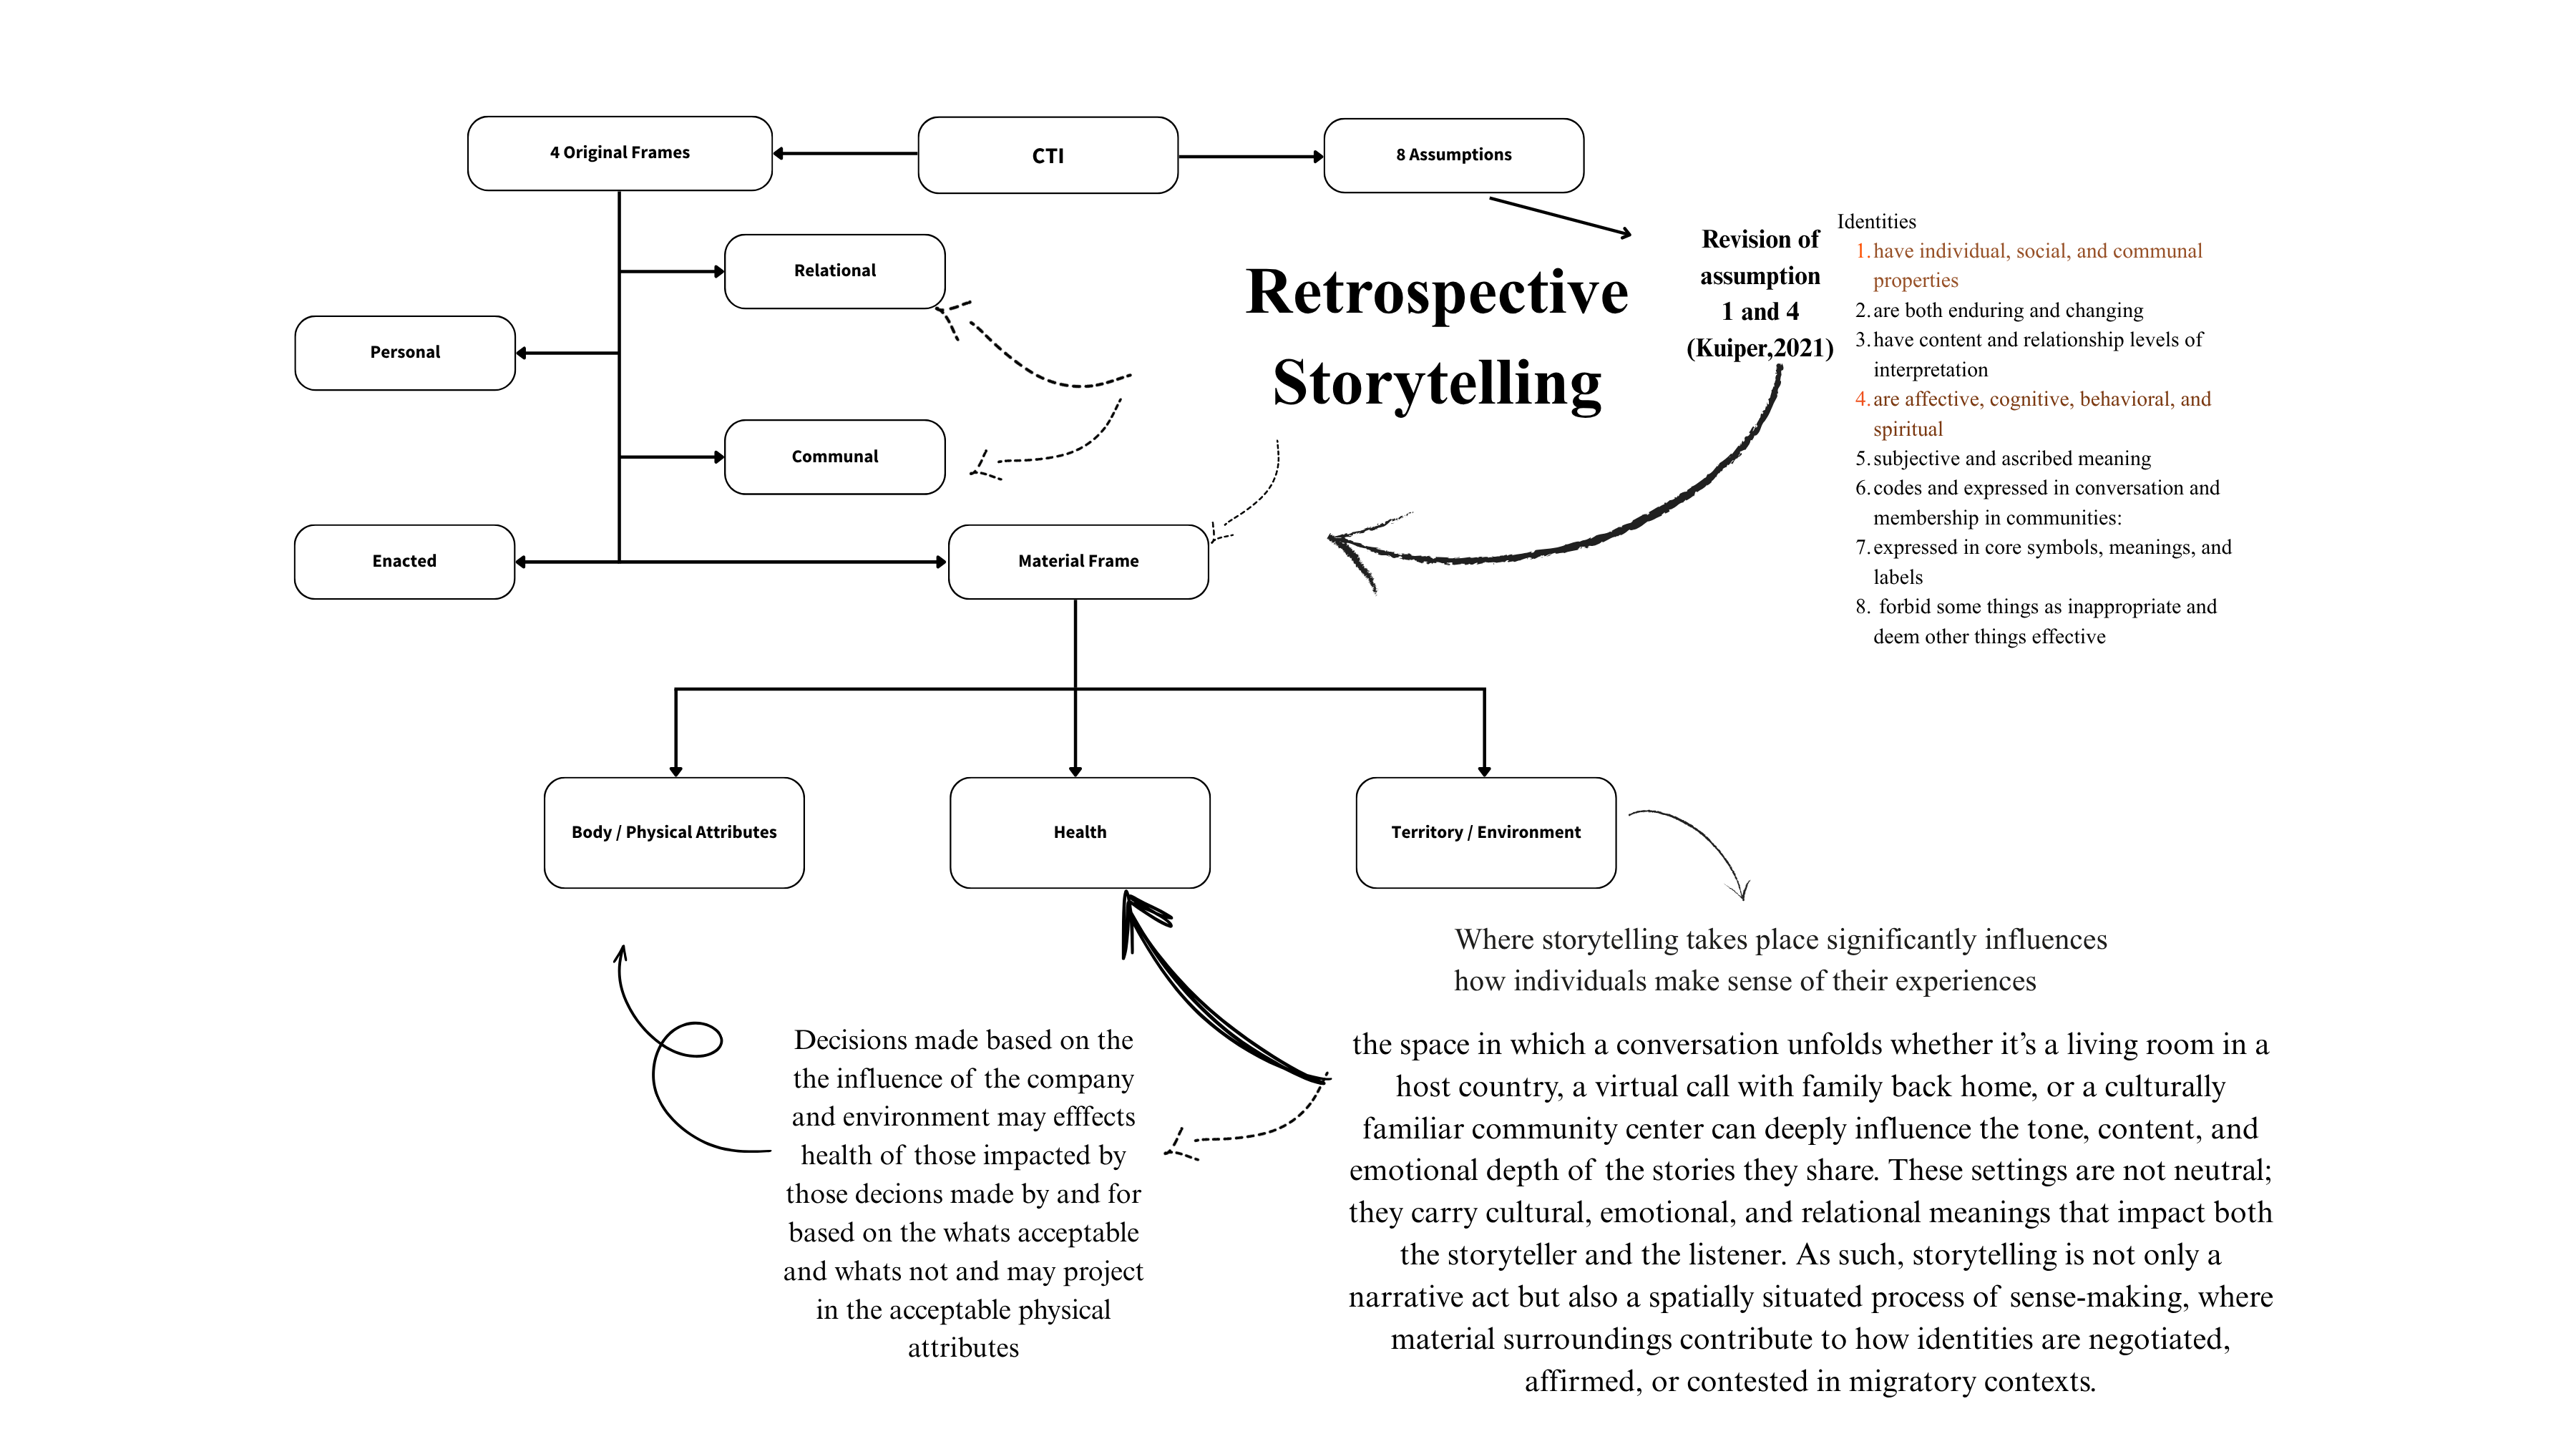
\includegraphics[width=1.0\linewidth,alt={A flowchart of the theoretical framework for the study}]{Dissertation/figures/Theoretical-Framework.png}
    \label{fig:theoretical-framework}
\end{figure}

\section{Poetry as a Tool of Analysis}

The study applied ABR methodology of poetic inquiry, which is used when the researcher's story intersects with or becomes entwined with the lives of research participants \citep{faulknerPoeticInquiryCraft2019} as well as to ``study identity, subjugated perspectives and difficult experiences'' \citep[p.~56]{faulknerExcavations2024}. It enabled me, as a researcher, to present more embodied experiences and evocative stories that can engage both academic and non-academic audiences. Poetic inquiry provided means to critically emphasize on personal experiences and sensitive personal narratives, enabling the fusion of scientific and humanistic perspectives on relationships through artistic forms \citep{ellingsonMakingDataQualitative2020, faulknerPoeticInquiryCraft2019, faulknerSettingAgendaPoetic2023, gioiachiltonArtsBasedResearchPractice2014}.

I employed poetic inquiry as both an analytic and representational tool (Faulkner, 2017). Poetic inquiry highlights the emerging prominent themes by developing poetic transcripts or found poems. Poetic transcripts are formed when the researchers transcribe participants' exact words from interviews to reveal lived experiences, keeping the original words and emotions intact \citep{faulknerPoeticInquiryCraft2019, faulknerSettingAgendaPoetic2023}.

This approach allowed me to preserve participants’ original voices while highlighting the emotional resonance embedded in their stories. Rather than reducing interviews into coded fragments alone, poetic inquiry illuminated the affective and embodied dimensions of participants’ accounts of family and lived experience. Through the construction of poetic transcripts, I was able to foreground not only spoken words but also the silences, pauses, and hesitations that carry profound meaning, elements that often risk erasure within conventional thematic analysis.

This analytic strategy enabled my commitment to honoring participants’ voices while acknowledging my interpretive role. Poetic transcription foregrounds the ``how'' of storytelling, drawing attention to the performative and relational qualities of narrative.

\section{Data Processing}

The process of data analysis began once interviews were conducted and recorded through Zoom Cloud. Zoom’s autogenerated transcripts provided the initial drafts, which were then carefully reviewed while listening to the audio recordings. Relevant edits were made to produce clean and accurate transcripts. In cases where conversations required translation or were rendered in Roman Urdu, efforts were made to preserve the originality of the participants’ voices. Where needed, transcripts were further translated and cleaned using AI tools i.e. ChatGPT \citep{naeemThematicAnalysisArtificial2025}. The AI tool was given specific passages that required translation, transcription, and formatting where the sudden switch between the languages was too frequent and Zoom transcripts were incomprehensible in any language. The AI tool-translated transcripts were read and tallied with the original recording to make final edits where the language needed adjustments to keep the emotions and meanings intact. For participants who declined to be recorded but still wished to share their experiences, only direct quotations given with consent were included, ensuring their voices were represented without leaving a digital footprint. 

This study adopted a nontraditional art-based approach to thematic analysis (i.e. poetic inquiry) to preserve and present the original words, voices, and emotions of participants. Past research shows that poetic inquiry provides marginalized voices with a platform through participatory, ethical, and multi-voiced processes aligned with social justice \citep{gioiachiltonArtsBasedResearchPractice2014}. Past scholars used poetic inquiry to present auto/ethnographic narratives of navigating their identities as immigrants, serving in military during wars, suffering of war, asylum seekers and refugees, as well as recoding life stories and oral biographical histories of older women \citep{faulknerPoeticPortraitureCritical2022, faulknerPoeticPortraitsOlder2026}. Guided by poetic inquiry, selected data was transformed into poetic transcripts (also called found poems) to fully convey the affective and embodied dimensions of experiences. The selection and arrangement of prose, pauses, line breaks, and spacing were used intentionally to foreground tension, emotions and meaning-making. As a part of analytical process, poetic analysis was conducted reflexively and in dialogue with the study’s theoretical framework. Selection and arrangement of the poetic transcripts functioned as an initial cycle of qualitative analysis rather than an aesthetic embellishment. 

Themes emerged through the poetic process itself. Each found poem was read as an analytic unit to identity recurring patterns of experience, emotion, and identity negotiation. As Faulkner argues, poetry enables researchers to recognize patterns through resonance and relationality, allowing meaning to surface through comparison rather than frequency \citep{faulknerPoeticInquiryCraft2019}. Through iterative reading and revision, clusters of poems revealed shared tensions, emotions, and guilt. These clusters established the basis for emergent themes that were articulated as poems accompanied with analytical narrative. Faulkner situates poetic inquiry as particularly aligned with feminist, narrative, and identity centered methodologies, emphasizing the importance of honoring complexity, embodiment, and partial truths. Accordingly, themes were interpreted not as fixed categories but as dynamic meaning-making processes situated within participants lived experiences \citep{faulknerPoeticInquiryCraft2019}.

\section{Researcher Preparation}

I listened to each audio recording multiple times, both before and after editing the autogenerated transcripts. This listening ensured transcription accuracy while also attuning me to the tones, pauses, and emotional inflections often lost in written text. Re-listening alongside the transcripts allowed for both accuracy checks and the identification of emerging impressions, recurrent images, and affective resonances. This practice was not just mechanical but reflective, enabling a deeper, embodied engagement with the data and strengthening the connection between analysis and lived experience.

As a researcher who is both embedded in and shaped by similar cultural contexts as my participants, I acknowledge my positionality in this process. My listening was never neutral but situated. Each return to the recordings became an exercise in both recognition and estrangement, hearing familiar experiences and cultural stories articulated through different voices, while also becoming aware of differences in generational location, gendered experiences, and individual personality. This recursive listening-reading-transcribing-relistening cycle prepared me to approach the next stage of analysis with both rigor and reflexivity.

In conclusion, the study adopted a qualitative art-based interpretative approach grounded in identity centered inquiry. Data was gathered through in-depth episodic narrative interviews and analyzed through thematic analysis using poetic inquiry. This methodological approach was intentionally selected to honor the participants lived experiences as Pakistani American immigrants while also advancing the theoretical insights. Moving forward, the following chapter presents the findings of this analysis.
